\documentclass[11pt]{article}

\usepackage[letterpaper,margin=1in]{geometry}
\usepackage{lipsum}

% ToC
\usepackage{blindtext} 
\usepackage[linktocpage]{hyperref}
\usepackage{bookmark}
\usepackage[compact]{titlesec}

% bib
%\usepackage[round]{natbib}
\usepackage[square,sort,numbers]{natbib}

% Math Imports
\usepackage{amsmath, amssymb, bm, fancyhdr, sectsty, dsfont, mathtools}

% Tikz
\usepackage{tikz}
\usetikzlibrary{bayesnet}
\usetikzlibrary{arrows}

\usepackage{wrapfig}
\usepackage{comment}
\usepackage{subcaption}
\usepackage{cleveref}

% Symbols
\newcommand\ind{\protect\mathpalette{\protect\independenT}{\perp}}
\def\independenT#1#2{\mathrel{\rlap{$#1#2$}\mkern2mu{#1#2}}}
\newcommand\norm[1]{\left\lVert#1\right\rVert}
\newcommand\set[1]{\left\{#1\right\}}

\newcommand\RNN{\mathrm{RNN}}
\newcommand\MLP{\mathrm{MLP}}
\newcommand\enc{\mathrm{enc}}
\newcommand\softmax{\mathrm{softmax}}

% Distributions
\newcommand{\Cat}{\mathrm{Cat}}
\newcommand\Expo{\mathrm{Expo}}
\newcommand\Bern{\mathrm{Bern}}
\newcommand\Pois{\mathrm{Pois}}
\newcommand\Bin{\mathrm{Bin}}
\newcommand\Unif{\mathrm{Unif}}
\newcommand\Betad{\mathrm{Beta}}
\newcommand\Gammad{\mathrm{Gamma}}
\newcommand\Geom{\mathrm{Geom}}
\newcommand\Logd{\mathrm{Logistic}}

\newcommand\E[1]{\mathbb{E}\left[#1\right]}
\newcommand\Es[2]{\mathbb{E}_{#1}\left[#2\right]}
\newcommand{\Var}{\mathrm{Var}}
\newcommand{\Cov}{\mathrm{Cov}}
\newcommand{\Cor}{\mathrm{Cor}}

% Bold stuff
\newcommand{\ba}{\mathbf{a}}
\newcommand{\bb}{\mathbf{b}}
\newcommand{\bc}{\mathbf{c}}
\newcommand{\bd}{\mathbf{d}}
\newcommand{\be}{\mathbf{e}}
\newcommand{\bg}{\mathbf{g}}
\newcommand{\bh}{\mathbf{h}}
\newcommand{\br}{\mathbf{r}}
\newcommand{\bs}{\mathbf{s}}
\newcommand{\bw}{\mathbf{w}}
\newcommand{\bx}{\mathbf{x}}
\newcommand{\by}{\mathbf{y}}
\newcommand{\bz}{\mathbf{z}}

% mathcal stuff
\newcommand{\mcD}{\mathcal{D}}

% math blackboard bold stuff
\newcommand{\R}{\mathbb{R}}
\newcommand{\C}{\mathbb{C}}
\newcommand{\Z}{\mathbb{Z}}
\newcommand{\N}{\mathbb{N}}
\newcommand{\Q}{\mathbb{Q}}


\DeclareMathOperator*{\argmin}{argmin}
\DeclareMathOperator*{\argmax}{argmax}

\titlespacing{\paragraph}{0pt}{*0}{*0}
%\setlength{\parskip}{-5mm plus1mm minus1mm}

\usepackage{fancyhdr}
\pagestyle{fancy}


\begin{document}
\lhead{Justin Chiu}
\chead{2018 NSF GRFP}
\rhead{Research Proposal}

\begin{center}
\textbf{Latent Variable Models for Data to Text Generation}
\end{center}

\paragraph{Keywords}
latent variable models, conditional text generation, data to text

\begin{comment}

\paragraph{Background}
Natural language processing (NLP) can largely be decomposed into two separate but
closely related tasks: natural language understanding and natural language
generation (NLG).
In this proposal we focus primarily on generation, and in particular
the generation of text that describes structured data.
We refer to this specific task as Data-to-Text (D2T).
The assumption that the text describes data is central to the task as it allows
for practitioners to define heuristics for evaluating a summary's fidelity to the
underlying data.

\paragraph{Why is D2T important?}
\begin{itemize}
\item Long-form generation but with structured input: a compromise between
short-form with unstructured inputs and long-form with unstructured inputs
\item Easily evaluable benchmark due to limited use of external knowledge
\end{itemize}
The D2T task's importance is two-fold.
First, D2T serves as a useful benchmark for conditional generation.
D2T exists as a compromise between short-form generative tasks such as sentence-level
translation and unstructured long-form tasks such as generating Wikipedia articles
from internet resources.
This is because D2T is a long-form generation task but uses structured data
as input instead of free-form text.
Secondly, the existence of structured data represents a simplifying assumption
which makes D2T easier than other long-form tasks but also, more importantly,
amenable to automatic evaluation.
Given a list of records and the assumption that in a data-text pair the text's purpose
is to describe the data,
it is straightforward to obtain possible alignments between the text and records for evaluation.
However, the alignments can also be used for much more than evaluation; they can be used for
obtaining weak supervision \citep{puduppully2018contentselection}.
%This insight motivates our proposal and will be elaborated on shortly.

\paragraph{What are the desiderata of a text generation system?}
\begin{enumerate}
% This is an iffy statement
\item Readability: Prior work has shown that models with fully connected observation models
in the form of a neural network result achieve higher BLEU scores than templated variants \citep{wiseman2017d2t},
which is correlated with readability.
\item Informational adequacy: This is decomposed into content selection and planning.
We can learn this directly as a model over
records as in \citep{puduppully2018contentselection}.
\item Fidelity to conditioning: We decompose factual errors into two types.
The first is the misalignment of records and the second is ignoring the record
completely and hallucinating values with a language model instead of copying them.
% Wow, so poorly phrased.
We posit that both errors are caused by insufficient conditioning of the
text given the records.
\citep{puduppully2018contentselection} attempts to address this by aligning
words to a content plan to provide more granular conditioning.
However, there are additional constraints that we know to be true:
the alignment between text and a record plan should be monotonic.
% Should I address this in more detail?
% Hypothesize that constraining the model results in sharper alignments
% and less noise, increasing fidelity to records
\item Controllability: 
Although a precise definition is available for dynamical systems,
we have yet to formalize a notion of controllability for NLG.
If we loosely define controllability as the ability to apply constraints during inference, 
latent variable models appear to be a viable approach.
We see this in \citep{puduppully2018contentselection}
as they can manipulate the model's content plan and control the generated summary.
By using oracle content plans extracted from the data,
they manage to obtain an upper bound on BLEU using only the raw data in the table.
\end{enumerate}

\paragraph{Current Trends}
Early work on D2T focused on the use of templates and grammars, 
which generally resulted in generations with little stylistic variation.
% Do I need to qualify this claim and say why?
After neural language models demonstrated state of the art performance,
they were then transferred to the conditional language modeling setting,
i.e. D2T and more broadly NLG,
where they supplanted template-based methods almost completely.
The result of using neural language models was an improvement in readability
at the cost of fidelity as well as controllability.
%However, by relying largely on the language modeling capabilities of neural networks,
%practitioners have eschewed modularity of the model for ease of inference.
% Do I need to qualify this as well?
%\citep{angeli2010d2t}, \citep{liang2009semalign}, \citep{sauper2009wiki}

\paragraph{Research Question}
%We can train end-to-end modular systems,
%so how much modularity and supervision can we provide and does it help the model?
As research on D2T has embraced neural systems and end-to-end training resulting
in very unstructured models, what is the benefit of imbuing more structure, namely in the
form of a hierarchical segmental model?
%As we add more complexity to our graphical model, what is the benefit of a latent variable model
%versus a soft approximation?
Using a hierarchical HSMM allows us to model
sentences in a modular and controllable way;
we can control the number of records referred to in a sentence and 
the structure of the sentence itself.
The formulation as a latent variable model allows us to enforce strict constraints on
the modeled characteristics (namely the number of reference records and sentence structure)
during inference, allowing a user to intervene during the text generation process.

\begin{wrapfigure}[22]{r}{0.45\textwidth}
\centering
\begin{subfigure}[]{0.4\textwidth}
\centering
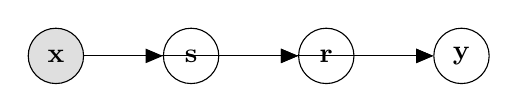
\begin{tikzpicture}
\node(x)[obs]{$\bx$};
\node(s)[latent, right =of x]{$\bs$};
\node(r)[latent, right =of s]{$\br$};
\node(y)[latent, right =of r]{$\by$};
\edge {x} {s};
\edge [bend right=30] {x} {r};
\edge {s} {r};
\edge [bend right=30] {s} {y};
\edge {r} {y};
\end{tikzpicture}
\label{tikz:simple}
\caption{}
\end{subfigure}

\begin{subfigure}[]{0.4\textwidth}
\centering
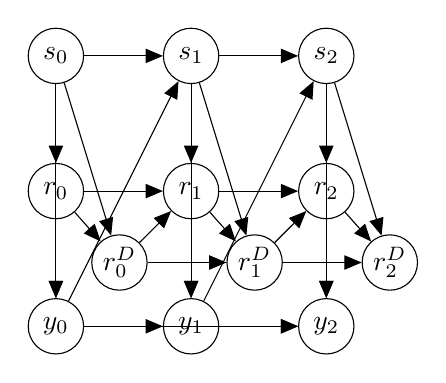
\begin{tikzpicture}
\node(s0)[latent]{$s_0$};
\node(r0)[latent, below =of s0]{$r_0$};
\node(r0d)[latent, below right =4mm and 3mm of r0]{$r_0^D$};
\node(y0)[latent, below =of r0]{$y_0$};
\node(s1)[latent, right =of s0]{$s_1$};
\node(r1)[latent, below =of s1]{$r_1$};
\node(r1d)[latent, below right =4mm and 3mm of r1]{$r_1^D$};
\node(y1)[latent, below =of r1]{$y_1$};
\node(s2)[latent, right =of s1]{$s_2$};
\node(r2)[latent, below =of s2]{$r_2$};
\node(r2d)[latent, below right =4mm and 3mm of r2]{$r_2^D$};
\node(y2)[latent, below =of r2]{$y_2$};

\edge {s0} {r0};
\edge [bend left=15] {s0} {r0d};
\edge [bend right=35] {s0} {y0};
\edge {r0} {y0};
\edge {r0} {r0d};

\edge {s1} {r1};
\edge [bend left=15] {s1} {r1d};
\edge [bend right=35] {s1} {y1};
\edge {r1} {y1};
\edge {r1} {r1d};

\edge {s2} {r2};
\edge [bend left=15] {s2} {r2d};
\edge [bend right=35] {s2} {y2};
\edge {r2} {y2};
\edge {r2} {r2d};

\edge {s0} {s1};
\edge {r0} {r1};
\edge {y0} {y1};
\edge {r0d} {r1};

\edge {r0d} {r1d};
\edge [bend left=15] {y0} {s1};

\edge {s1} {s2};
\edge {r1} {r2};
\edge [bend right=25] {y0} {y2};
\edge {y1} {y2};
\edge {r1d} {r2};

\edge {r1d} {r2d};
\edge [bend left=15] {y1} {s2};


\end{tikzpicture}
\label{tikz:full}
\caption{}
\end{subfigure}
\label{fig:pgm}
\caption{
(a) is a simplified graphical representation of the model
that ignores the temporal dependencies.
$\bx$ is the input data, $\bs$ the style, $\br$ the content,
and $\by$ the words of the summary.
(b) is the full graphical model.
We leave out conditioning on $\bx$ for brevity.
The new variables $r_i^D$ represent the duration a record is used.
}
\end{wrapfigure}
\paragraph{Argument for LVM}
\begin{enumerate}
\item The fully neural approach in \citep{puduppully2018contentselection} takes the output of
an information extraction system as the ground truth and trains a content planning model with
that assumption.
Any mistakes in the information extraction system will be replicated in the final model.
%In addition, the information extraction is trained via a heuristic alignment
%procedure that aligns words that appear in the database to records containing those words. 
%However, we argue that this particular procedure results in a compounding of mistakes.
% should use more precise notation here
Thus we argue that training the information extraction system by incorporating it
into an approximate posterior will improve performance as measured by
the likelihood of the data under our model.
\item As demonstrated in \citep{liang2009semalign},
a structured LVM results in qualitatively better segmentations than an unstructured one.
The latent variable formulation allows us to impose different inductive biases than a 
purely neural model.
For example, \citep{liang2009semalign} enforce monotonic alignments between text and records by using a 
hidden semi-markov model (HSMM).
\item Convincing templates from prior work \citep{wiseman2018template} indicate that the separation of
style and content is plausible.
\item Explicitly modeling characteristics such as the number of records in a given
sentence is possible in a latent variable model such as a HSMM.
\end{enumerate}

\paragraph{Data}
% Example of D2T, should i present this early or later
The dataset we focus on is the Rotowire dataset \citep{wiseman2017d2t},
where a summary of a basketball game is modelled conditioned on the box score
associated with that game.
This is the most recent D2T dataset that has been developed.
The box score consists of a list of records associating an entity with a value.
Each record has a type which denotes the relationship between the entity and value
contained in the record,
for example: (type = POINTS, entity = Jeremy Lin, value = 19).
We learn a model that generates the summary conditioned on the box score.
The model is evaluated based on its fidelity to data and
is also compared to a human-generated summary in terms of which records are chosen,
their order, as well as the n-gram overlap of the summaries themselves.

\paragraph{Approach and Methods}
% Proposal? Add more structure / modularity, principled inference...?
% Thesis: structure will help with controllability and LVM formulation
% with generalization as it presents a different inductive bias?
We would like to unify works from several directions:
\begin{enumerate}
\item Structure away content modeling through templates
\citep{sauper2009wiki,wiseman2018template}
\item Content planning and incorporating weak supervision
\citep{puduppully2018contentselection}
\item Efficient training methods for discrete LVMs \citep{deng2018vattn}
\end{enumerate}
% Elaborate on each of those points
We propose to model the conditional distribution of a summary given data as a 
hierarchical HSMM, as in \citep{liang2009semalign}.
Ignoring the temporal aspect of the model, we define a simplified model
with the following parts:
\begin{enumerate}
\item The given structured data $\bx$ 
\item Each sentence is generated using a style $s_i$
\item The content in each sentence $\br_i$ is chosen from $\bx$
after choosing a style $s_i$
\item The words in the summary $y_i$ are chosen conditioning on
the current content from $r_i$ as well as the style $c_i$
\end{enumerate}
We also present a more detailed model:
% Caveat: we don't want r_t to depend on r_{t-1} if starting a new sentence.
\begin{enumerate}
\item The style features $s_t\mid y_{t-1},s_{t-1},\bx\sim\Cat()$
\item The record choices $r_t\mid r_{t-1}^D,r_{t-1},s_t,\bx\sim\Cat()$
\item The record duration is given by 
$r_t^D\mid r_{t-1}^D=0,r_t\sim\Unif(1,\ldots,L)$
where $L$ is the max segment length and $r_t^D\mid r_{t-1}^D=x = x-1$

\item The words in the summary $y_t\mid y_{<t},r_t,s_t\sim\Cat()$
\end{enumerate}
See Figure~\ref{fig:pgm} for a simplified graphical depiction of the model.
We include a fully-specified slice of the time-series model as well,
but do not elaborate on it.

% too expensive to align to records since there may be many of them
As defined, the model would be very expensive to train via maximum marginal likelihood
training. We therefore propose to use the method proposed in \citep{deng2018vattn}
in order to make training tractable: namely define a variational approximation to the
posterior and use REINFORCE to maximize a lower bound on the marginal likelihood.
We also propose to incorporate intermediate weak supervision in the form of
heuristic record-to-text alignments.

% Should I explain why I propose a LVM versus a fully discriminative model?
% 
\paragraph{Intellectual Merit}
We hope to demonstrate the benefits of a hierarchical model in the task of text generation.
We propose a structure-aware content model similar to
work in \citep{sauper2009wiki,wiseman2017d2t,liang2009semalign}
that incorporates the computational advances in \citep{deng2018vattn}
in order to scale training.

\paragraph{Broader Impact}
The task of D2T itself is important, rather than simply a compromise between
short and long-form generation tasks.
Given a complicated set of structured data with possibly many records
which are irrelevant, an ideal D2T system would perform information triage by 
picking salient records then organize those records into prose.
This would be much easier to understand for someone unfamiliar with the
particular structure of the data and would aid in the dissemination of 
technological understanding.
With an interpretable LVM the user would also be able to examine the aligned
records that generated the summary, allowing the user to learn to read
the data by following the system's example.
% Stretch
\end{comment}

\section{Outline}
\begin{enumerate}
\item Background
\begin{enumerate}
\item Breakdown of NLP into NLU and NLG
\item Importance of D2T, an instance of NLG
\begin{enumerate}
\item A compromise between short-form and long-form conditional generation  
\item Easily evaluable benchmark due to limited use of external knowledge
\item Convenient representation of input allows us to isolate
progress on generation metrics
\end{enumerate}
\item Introduce Rotowire \citep{wiseman2017d2t}
\begin{enumerate}
\item A summary of a basketball game is modelled conditioned on the box score
associated with that game.
\item The box score consists of a list of records associating an entity with a value.
Each record has a type which denotes the relationship between the entity and value
contained in the record,
for example: (type = POINTS, entity = Jeremy Lin, value = 19).
\end{enumerate}
\item Desiderata of Text Gen Systems, and how they are measured
\begin{enumerate}
\item Readability: How easy is it for a human to read the generated summary?
Refers to fluency and grammaticality, and is with BLEU as the two have been
shown to be correlated {cite BLEU paper}.
\item Informational Adequacy: How well does the model recreate the informational content
of a human-generated summary?
Measured through metrics concerning the selection and ordering of records.
\item Fidelity to conditioning: 
A lack of fidelity occurs if the model either ignores the data input and hallucinates
a value through the language model or if the model misaligns a record to a given segment of text.
\item Controllability:
Although a precise definition is available for dynamical systems,
we have yet to formalize a notion of controllability for NLG.
We loosely define controllability as the ability to apply constraints during inference.
\end{enumerate}
\item Current trends addressing desiderata
\begin{enumerate}
\item Initially research focused largely on readability,
and improved on BLEU scores through the use of conditional neural language models.
Compared to template-based methods, summaries were more fluent and natural.
However, by removing structure from the model and relying on the flexibility of neural networks
informational adequacy, fidelity, and controllability were sacrificed \citep{wiseman2017d2t}.
\item Follow-up work re-introduced the explicit modeling of content
\citep{puduppully2018contentselection}, which improved on informational adequacy and
fidelity to conditioning through a latent content plan.
Although not entirely explored in the aforementioned work,
modeling the content plan also affords a degree of controllability.
By using oracle content plans extracted from the data,
they manage to obtain an upper bound on BLEU using only the raw data in the table.
\end{enumerate}
\end{enumerate}
\item Research Question
\begin{enumerate}
\item As research on D2T has embraced neural systems and end-to-end training
resulting in very unstructured models,
what is the benefit of imbuing more structure,
namely in the form of a hierarchical segmental model?
For the task of data-to-text, using a hierarchical HSMM allows us to model sentences
in a modular and controllable way;
we can control the number of records referred to in a sentence and the structure
of the sentence itself.
The formulation as a latent variable model allows us to enforce strict constraints on
the modeled characteristics (namely the
number of reference records and sentence structure) during the text generation process.
\end{enumerate}
\item Argument for a LVM:
Although the argument for modularity applies equally to models expressible as
neural networks as well as latent variable models, LVMs allow us to:
\begin{enumerate}
\item Learn an information extraction system jointly with the generative model.
\item Encode different inductive biases than neural models due to the ability to make hard decisions
and enforce structure.
\item Utilize weak supervision in a principled way.
\end{enumerate}
\item Approach and Methods
\begin{enumerate}
\item Structure-aware content selection \citep{sauper2009wiki}
through a hierarchical HSMM \citep{wiseman2018template}.
\item Weak supervision for the content planning model and information extraction model
through posterior constraints.
\end{enumerate}
\end{enumerate}

\bibliographystyle{plainnat}
\bibliography{w}

\end{document}

